\section{Introduction}
\label{sec:intro}

% \begin{tight_itemize}
%   \item Introduce the problem
%   \item Describe our approach
%   \item Contrast with Milan's work
%   \item Contrast with Andreas Geiger's work
%   \item Highlight the contributions
% \end{tight_itemize}
% \vspace{10cm}

        To accomplish fully or partial autonomous driving we need 3D
        localization of traffic participants in the scene. 
        Since laser scanners and stable wide--baseline stereo setups are
        expensive, we focus on solving the problem using monocular video, GPS
        and maps as our input. Given the video we extract detection bounding
        boxes, ground plane and point tracks.
        We formulate the problem of 3D localization in a probabilistic graphical
        model specifically a factor graph model. We use additional heuristic
        constraints like collision constraint, that leads to a global consistent solution.
        Using these multiple sources of information that provide, possibly conflicting, evidence about
        the location of traffic participant, a consistent meaningful solution must be estimated. 
        We formulate the problem in factor graph
        formalism and use off-the-shelf methods for inference.

        Our work is quite similar to that of Milan et
        al~\cite{Milan_etal_2014}, except that we provide a optics based
        perspective to occlusion modeling and our modeling is more detailed
        than that used in Milan et al. In terms of application we perform 3D
        localization using monocular camera while \cite{Geiger_etal_2014} use
        stereo for similar results.

\begin{figure}[!!t]
  %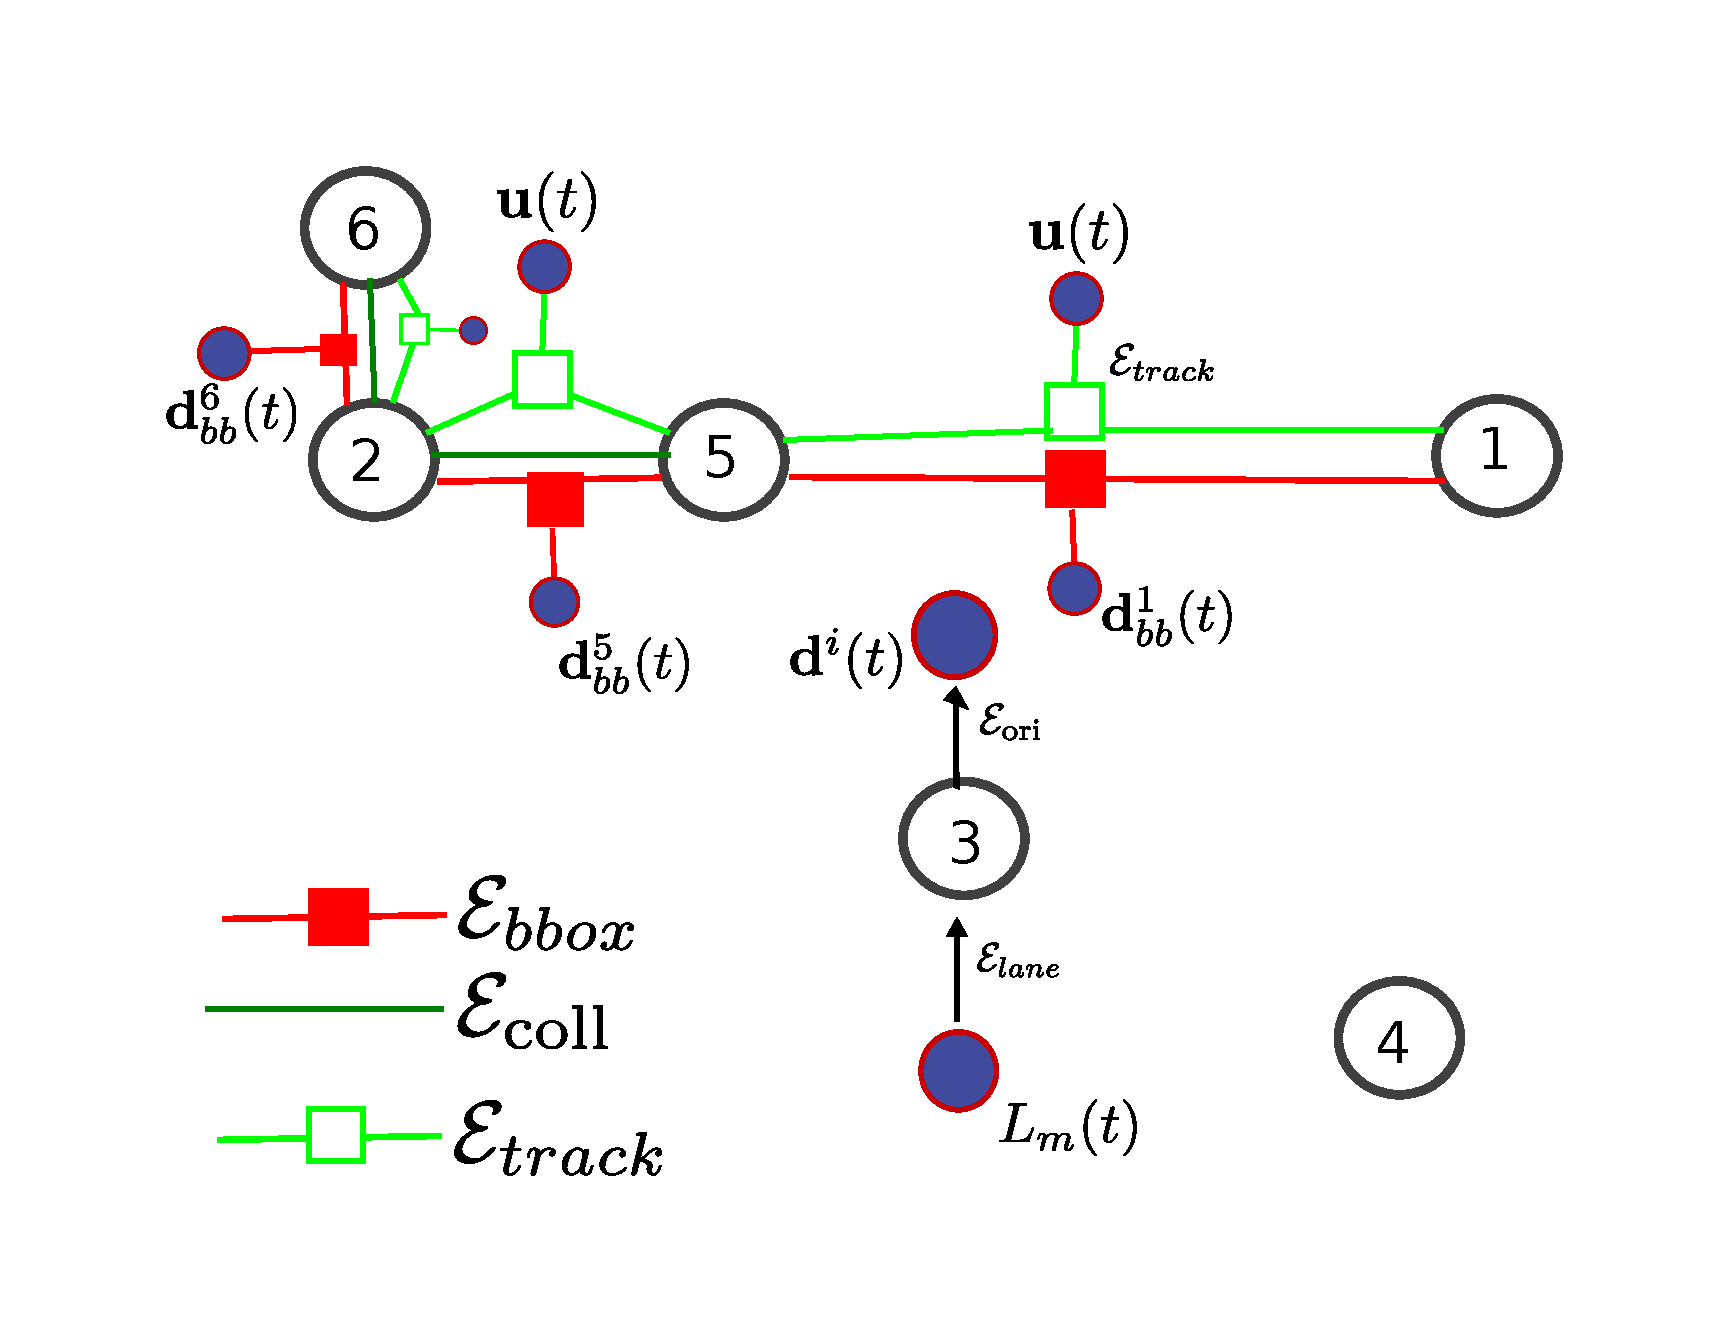
\includegraphics[width=\columnwidth]{Figures/graphicalModelFrom61ConstVars.pdf}
  \begin{center}
  \usetikzlibrary{trees,shadows}
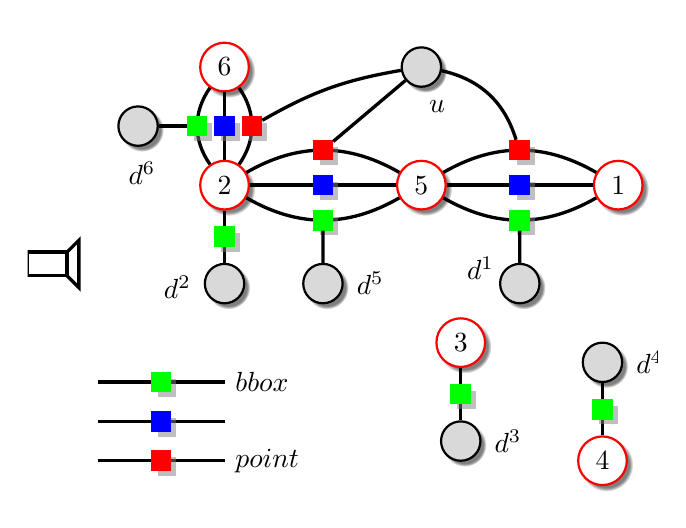
\begin{tikzpicture}[grow cyclic, line width=1.2pt,
    variablenode/.style={circle,circular drop shadow,draw=red,fill=white,thick,minimum width=0.5cm},
   bboxfactor/.style={rectangle,drop shadow,draw=green,fill=green,thick,minimum width=0.2cm},
    collfactor/.style={rectangle,drop shadow,draw=blue,fill=blue,thick,minimum width=0.2cm},
    trackfactor/.style={rectangle,drop shadow,draw=red,fill=red,thick,minimum width=0.2cm},
  obs/.style={fill=gray!30,draw=black},
  prevf/.style={draw=green!20,text=gray},
  prevobsv/.style={draw=gray!10,fill=gray!1,text=gray},
  prevv/.style={draw=red!20,text=gray}
]
  \path[use as bounding box,clip] (-2.5, -5.5) rectangle (5.5,0.5);
  \draw (-2.5,-2.65) rectangle +(0.5,0.3);
  \draw (-2.0,-2.35) -- ++(0.15, 0.15) -- ++(0, -0.6) -- (-2.0, -2.65);
\path
     (0, 0)  node [variablenode] (x6) {6}
++(0, -1.5) node [variablenode] (x2) {2}
++(2.5, 0)  node [variablenode] (x5) {5}
+ (0, 1.5)  node [variablenode,obs] (u) {}
+(.2,1.0)  node {$u$}
+ (.5, -2)   node [variablenode] (x3) {3}
+ (2.3, -3.5)   node [variablenode] (x4) {4}
+(2.5, 0)  node [variablenode] (x1) {1}
;

% Factors between nodes 6 and 2
\draw (x6) edge [bend right=35] node [bboxfactor] (f26) {} (x2);
\path (f26) +(-0.75,0) node [variablenode,obs] (d6) {} 
                        +(-.7,-.6)  node {$d^6$};
\draw (f26) edge (d6);
\draw (x6) edge [bend left=35] node [trackfactor] (ft26) {} (x2);
\draw (ft26) edge [bend left=10] (u);
\draw (x6) edge node [collfactor] {} (x2);

% Factors for node 2
\path (x2) +(0,-1.25) node [variablenode,obs] (d2) {} 
                        +(-.6,-1.3)  node {$d^2$};
\draw (x2) edge node [bboxfactor] {} (d2);

% Factors between nodes 2 and 5
\draw (x2) edge [bend right] node [bboxfactor] (f25) {} (x5);
\draw (x2) edge [bend left] node [trackfactor] (ft25) {} (x5);
\draw (x2) edge [] node [collfactor] {} (x5);
\draw (ft25) edge (u);
\path (x5) ++(-1.25,-1.25) node [variablenode,obs] (d5) {} 
                        +(.6,0)  node {$d^5$};
\draw (f25) edge (d5);

% Factors between nodes 5 and 1
\draw (x5) edge [bend right] node [bboxfactor] (f51) {} (x1);
\draw (x5) edge [bend left] node [trackfactor] (ft51) {} (x1);
\draw (x5) edge [] node [collfactor] {} (x1);
\draw (ft51) edge [bend right] (u);
\path (x1) ++(-1.25,-1.25) node [variablenode,obs] (d1) {} 
                        +(-.5,0.2)  node {$d^1$};
\draw (f51) edge (d1);

% Factors for node 3
\path (x3) ++(0,-1.25) node [variablenode,obs] (d3) {} 
                        +(.6,0)  node {$d^3$};
\draw (x3) edge node [bboxfactor] {} (d3);

% Factors for node 4
\path (x4) ++(0,1.25) node [variablenode,obs] (d4) {} 
                        +(.6,0)  node {$d^4$};
\draw (x4) edge node [bboxfactor] {} (d4);

% Legend
\path (-1.75,-4.0) node (l1s) {} (-0, -4.0) node [anchor=west] (l1e) {$\Energy{bbox}$};
\draw (l1s) edge node [bboxfactor] {} (l1e);
\path (-1.75,-4.5) node (l2s) {} (0, -4.5) node [anchor=west] (l2e) {$\EnergyCol$};
\draw (l2s) edge node [collfactor] {} (l2e);
\path (-1.75,-5.0) node (l3s) {} (0, -5.0) node [anchor=west] (l3e) {$\Energy{point}$};
\draw (l3s) edge node [trackfactor] {} (l3e);

\end{tikzpicture}

  \end{center}
  \caption{Graphical model. The six numbered black circles represent the
    unknown state variables of each car. All other nodes in the graphical model
    are assumed
    observed variables. Consider each energy in the model one by one. (1)
    Bounding box energy: The bounding box energy without occlusion modeling is
    a unary term, but with occlusion it becomes a higher order term that
    affects the state of occluder as well. In this graphical model we assume
    that the scene is being observed from left to right, hence "2" occludes "6"
    and "5" and "5" occludes "1". The bounding box detection is represented by
  $\mathbf{d}_{bb}^i(t)$ and the statistical dependencies are represented by
  red lines. (2) Point tracks ($\Energy{track}$): Since occlusion is also
  included in modeling point tracks energy we have similar interdependencies
  for point tracks energy. The available point tracks are modeled by
  $\mathbf{u}(t)$. (3) Collision ($\Energy{coll}$) : The collision energy
  mathematically is a dense graph between all the TP but here we represent
  collision among only those TP that are near enough to have a significant
collision energy. (4) Orientation from detection ($\Energy{ori}$) (5) Orientation from lane (and map) information ($\Energy{lane}$)}
  \label{fig:graphmodel}
\end{figure}
\begin{figure}
  \centering
    	  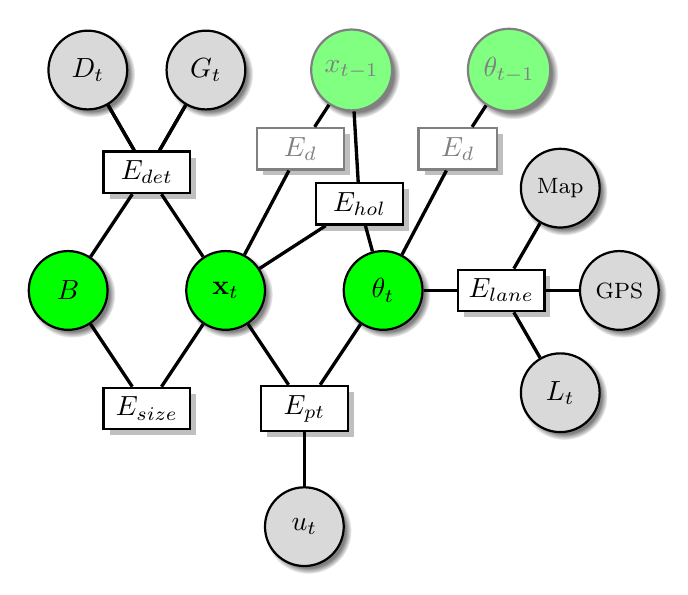
\begin{tikzpicture}[grow cyclic,line width=1.2pt,
variablenode/.style={circle,circular drop shadow,draw=black,fill=green,thick,minimum width=1.0cm},
  	  factor/.style={rectangle,drop shadow,draw=black,fill=white,thick,minimum width=1.1cm},
      obs/.style={fill=gray!30},
      prev/.style={text=gray,draw=gray,fill=green!50}]
  	  \path 

(0.6,2.8) node [variablenode,prev] (xt1) {$x_{t-1}$}
(2.6,2.8) node [variablenode,prev] (theta1) {$\theta_{t-1}$}

(-0.05,1.8) node [factor,draw=gray,text=gray] (fdynx) {$E_{d}$}
(1.95,1.8) node [factor,draw=gray,text=gray,minimum width=1cm] (fdynt) {$E_{d}$}

(.7,1.1) node[factor](fhol) {$E_{hol}$}

  	 (1, 0)  node[variablenode](theta){$\theta_t$}
   [counterclockwise from=-60,sibling angle=60]
     (2.5, 0) node [factor] (flane) {$E_{lane}$} 
    child { node [variablenode,obs] (l) { $L_t$ } }
    child { node [ variablenode,obs,font=\footnotesize] (gps) {GPS}}
    child { node [ variablenode,obs,font=\footnotesize] (gps) {Map}}
  	(-1, 0)  node[variablenode](xt){$\mathbf{x}_t$}

    [counterclockwise from=60,sibling angle=60]
  	(-2, 1.5) node[factor](fdet){$E_{det}$} 
  	           child {
  	             node[variablenode,obs](gp){$G_t$} 
  	  			}
	  	   		child {           node[variablenode,obs](Det){$D_t$}
  			  }

      (-2.0,-1.5) node[factor](fsize){$E_{size}$}
     (-3,0) node[variablenode](dim){$B$}
[counterclockwise from=-90]
 (0, -1.5) node[factor](fpt) {$E_{pt}$}
 child { node[variablenode,obs](pt){$u_t$} }


  	  ;
  	  \draw (xt) -- (fdet) -- (Det);
  	  \draw (xt) edge (fpt);
      \draw (fpt) -- (pt);
  	  \path  (fpt) edge (theta);
  	  \draw (fdet) -- (gp);
      \draw (fhol) -- (xt);
      \draw (fhol) -- (xt1);
      \draw (fhol) -- (theta);  	  
      \draw (dim) -- (fdet);
     \draw (xt) -- (fsize) -- (dim);
   \draw (theta) -- (flane);
   \draw (xt) -- (fdynx) -- (xt1);
   \draw (theta) -- (fdynt) -- (theta1);
	\end{tikzpicture}

\end{figure}
